\documentclass[10pt,a4paper]{article}

%% paquetes basicos
\usepackage[utf8]{inputenc}
\usepackage[spanish]{babel}
\usepackage{a4wide,color,verbatim,Sweave,url,xargs,amsmath,booktabs,longtable}
\usepackage{graphicx,float}
\usepackage{tikz,xcolor}
\usepackage{enumitem}

%% bibliotecas TikZ
\usetikzlibrary{automata,positioning,calc,arrows}

%% entornos para exams
\newenvironment{question}{\item}{}
\newenvironment{solution}{\comment}{\endcomment}
\newenvironment{answerlist}{\renewcommand{\labelenumii}{(\alph{enumii})}\begin{enumerate}}{\end{enumerate}}

%% comandos para metadatos exams
\newcommand{\exname}[1]{\def\@exname{#1}}
\newcommand{\extype}[1]{\def\@extype{#1}}
\newcommand{\exsolution}[1]{\def\@exsolution{#1}}
\newcommand{\exshuffle}[1]{\def\@exshuffle{#1}}
\newcommand{\exsection}[1]{\def\@exsection{#1}}

%% configuracion parrafos
\setlength{\parskip}{0.7ex plus0.1ex minus0.1ex}
\setlength{\parindent}{0em}

\begin{document}
\Sconcordance{concordance:costo_boleta_orig_interpretacion_representacion_n2_v1.tex:costo_boleta_orig_interpretacion_representacion_n2_v1.Rnw:1 %
33 1 1 169 32 1 1 4 1 1 1 4 1 1 1 4 1 1 1 4 13 1 1 2 4 0 1 2 11 1}


\begin{enumerate}


\begin{question}

El costo de la boleta en un cine depende de la edad de la persona, mientras que el costo de las palomitas se mantiene fijo. La siguiente tabla muestra la relacion entre estas dos variables:

\begin{center}
\begin{tabular}{|c|c|}
\hline
\textbf{Costo de entrada (x)} & \textbf{Costo de bebida (y)} \\
\hline
0 & 11000 \\
\hline
8 & 10000 \\
\hline
16 & 9000 \\
\hline
24 & 8000 \\
\hline
32 & 7000 \\
\hline
40 & 6000 \\
\hline
48 & 5000 \\
\hline
56 & 5000 \\
\hline
\end{tabular}
\end{center}

La grafica que representa esta funcion es:

\begin{answerlist}
\item
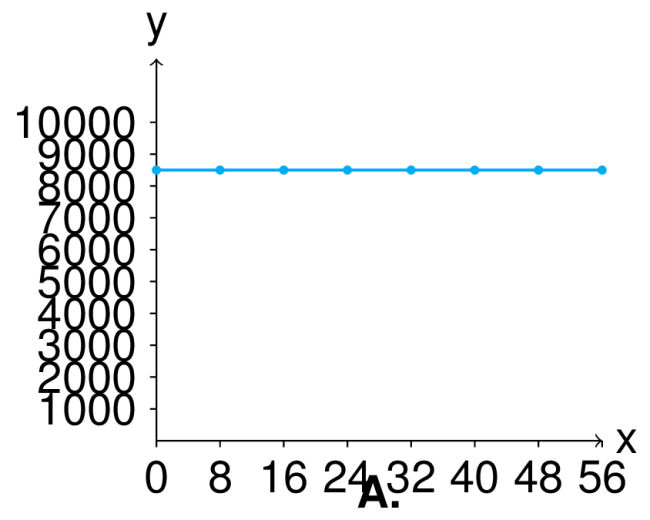
\includegraphics[width=6cm]{graficaA.png}
\item
\includegraphics[width=6cm]{graficaB.png}
\item
\includegraphics[width=6cm]{graficaC.png}
\item
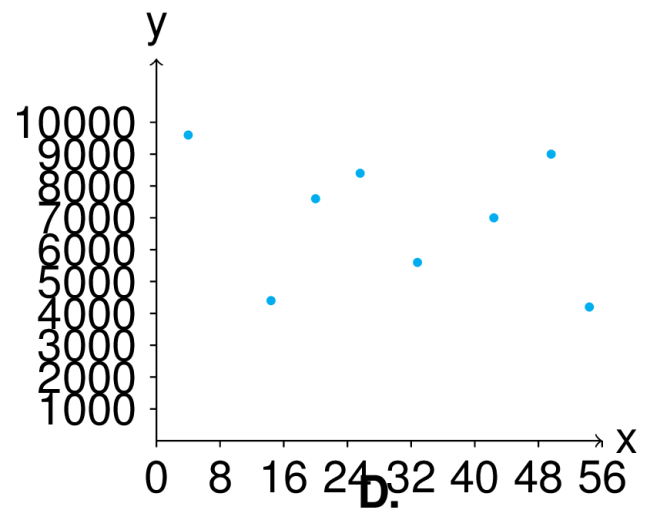
\includegraphics[width=6cm]{graficaD.png}\end{answerlist}

\end{question}

\begin{solution}

Para resolver este problema, debemos analizar la relacion entre las dos variables presentadas en la tabla.

Observando los datos:
- Cuando el entrada cuesta $0$, el bebida cuesta $11000$
- Cuando el entrada cuesta $56$, el bebida cuesta $5000$

Esto muestra una relacion lineal decreciente entre las variables.

\begin{answerlist}
  \item Falso. La grafica A muestra una relacion constante, no la relacion decreciente mostrada en la tabla.
  \item Verdadero. La grafica B representa correctamente la relacion lineal decreciente mostrada en los datos.
  \item Falso. La grafica C muestra una funcion escalonada, no una relacion lineal continua.
  \item Falso. La grafica D muestra puntos dispersos sin conexion, no una funcion definida.
\end{answerlist}
\end{solution}

%% META-INFORMATION
\exname{Costo Boleta Original Interpretacion Representacion}
\extype{schoice}
\exsolution{0100}
\exshuffle{TRUE}
\exsection{Interpretacion y Representacion}

\end{enumerate}
\end{document}
